% Dieser Text ist urheberrechtlich gesch\"utzt
% Er stellt einen Auszug eines von mir erstellten Referates da
% und darf nicht gewerblich genutzt werden
% die private bzw. Studiums bezogen Nutzung ist frei
% April 2011
% Autor: Sascha Frank 
% Universit\"at Freiburg 
% www.informatik.uni-freiburg.de/~frank/
% frank < was da sonst immer steht > tf.uni-freiburg.de


\documentclass[hyperref={pdfpagelabels=false}]{beamer}
% Die Hyperref Option hyperref={pdfpagelabels=false} verhindert die Warnung:
% Package hyperref Warning: Option `pdfpagelabels' is turned off
% (hyperref)                because \thepage is undefined. 
% Hyperref stopped early 
%

\usepackage{lmodern}
% Das Paket lmodern erspart die folgenden Warnungen:
% LaTeX Font Warning: Font shape `OT1/cmss/m/n' in size <4> not available
% (Font)              size <5> substituted on input line 22.
% LaTeX Font Warning: Size substitutions with differences
% (Font)              up to 1.0pt have occurred.
%

% Wenn \titel{\ldots} \author{\ldots} erst nach \begin{document} kommen,
% kommt folgende Warnung:
% Package hyperref Warning: Option `pdfauthor' has already been used,
% (hyperref) ... 
% Daher steht es hier vor \begin{document}

\title{Nichtparametrische Regression durch tiefe neuronale Netzwerke mit ReLU Aktivierungsfunktion }   
\author{Minh Duc Bui} 
\date{\today} 

% zusaetzlich ist das usepackage{beamerthemeshadow} eingebunden 
\usepackage{beamerthemeshadow}

%  \beamersetuncovermixins{\opaqueness<1>{25}}{\opaqueness<2->{15}}
%  sorgt dafuer das die Elemente die erst noch (zukuenftig) kommen 
%  nur schwach angedeutet erscheinen 
\beamersetuncovermixins{\opaqueness<1>{25}}{\opaqueness<2->{15}}
% klappt auch bei Tabellen, wenn teTeX verwendent wird\ldots

\usepackage{mathtools}

\begin{document}
\newcommand{\E}{\mbox{I\negthinspace E}}
\newcommand{\RN}[1]{\uppercase\expandafter{\romannumeral#1}}
\DeclarePairedDelimiter{\abs}{\lvert}{\rvert} 
\DeclarePairedDelimiter{\norm}{\lVert}{\rVert}
\newcommand{\argmin}{arg\,min}

\AtBeginSection[]{
  \begin{frame}
  \vfill
  \centering
  \begin{beamercolorbox}[sep=8pt,center,shadow=true,rounded=true]{title}
    \usebeamerfont{title}\insertsectionhead\par%
  \end{beamercolorbox}
  \vfill
  \end{frame}
}



\begin{frame}
\titlepage
\end{frame} 

\begin{frame}[allowframebreaks]
\frametitle{Inhaltsverzeichnis}
\tableofcontents
\end{frame} 


\section{Einleitung} 


\subsection{Ziel der Arbeit}
\begin{frame} 
\frametitle{Ziel der Arbeit}  
Annahme: Multivariates nichtparametrisches Regressionsmodel und  die Regressionsfunktion besteht aus einer Komposition von Funktionen. Betrachten ein \textit{sparsly connected} tiefes neuronales Netzwerk mit einer ReLU Aktivierungsfunktion. \\Ziele:
\begin{itemize}
\item Für eine bestimmte gewählte Netzwerkarchitektur, eine obere Schranke für den $L_2$-Fehler beweisen
\item Untere Schranke für $L_2$-Fehler angeben
\item Minimax-Konvergenzrate für Schätzer aus solchen Netzwerken
\end{itemize}
\end{frame}

\subsection{Nichtparametrische Regression}
\begin{frame}
\frametitle{Nichtparametrische Regression \RN{1}}
\begin{itemize}
\item Zufallsvektor $(\mathbf{X},Y)$ mit Werten in $\mathbb{R}^d \times \mathbb{R}$, wobei $\E Y^2 < \infty$
\item  $Y = f(\mathbf{X}) + \epsilon$, wobei Störgröße standardnormalverteilte und unabhängig von $\mathbf{X}$  Zufallsvariable
\item Minimiere $\E[L(Y,f'(\mathbf{X}))]$, wobei $L: \mathbb{R} \times \mathbb{R} \rightarrow \mathbb{R}_{\geq 0}$ messbare Funktion
\item Wähle $L(y,s) = (y-s)^2$ quadratische Verlustfunktion, es folgt $\E[\vert Y - f'(\mathbf{X})\vert ^2]$
\end{itemize}
\end{frame}

\begin{frame}
\frametitle{Nichtparametrische Regression \RN{2}}
\begin{itemize}
\item $m:\mathbb{R}^d \to \mathbb{R},\ m = \E (Y \vert \mathbf{X} = \mathbf{x})$ nennt man Regressionsfunktion
\item $\E (\vert f'(\mathbf{X})-Y\vert^2) = \E (\vert f'(\mathbf{X}) - m(\mathbf{X})) \vert ^2 ) + \E (\vert m(\mathbf{X}) - Y) \vert ^2 )$
\item $\E (\vert f'(\mathbf{X}) - m(\mathbf{X})) \vert ^2 )$ nennt man $L_2$-Fehler von $f'$
\item Regressionsfunktion minimiert $L_2$-Fehler, aber nicht berechenbar
\end{itemize}
\end{frame}

\begin{frame}
\frametitle{Nichtparametrische Regression \RN{3}}
\begin{itemize}
\item Gegebene Beobachtungen $D_n = {(\mathbf{X}_1, Y_ 1, ..., \mathbf{X}_n,Y_n)}$, wobei $(\mathbf{X},Y), (\mathbf{X}_1, Y_ 1), ..., (\mathbf{X}_n,Y_n)$ u.i.v. Zufallsvariablen 
\item Ziel: $f_n(\mathbf{x}) = f_n(\mathbf{x},D_n)$ konstruieren, sodass die $L_2$-Fehler 
\begin{equation*}
\E (\vert f_n(\mathbf{X})-f_0(\mathbf{X})\vert^2) = \int \vert f_n(\mathbf{x})-f_0(\mathbf{x})\vert ^2 P _X(dx)
\end{equation*} minimal 
\end{itemize}
\end{frame}

\subsection{Konvergenzrate}
\begin{frame}
\frametitle{Konvergenzrate \RN{1}}
\begin{itemize}
\item Definiere $L_2$ Fehler als $R( f_n, f_0) := \int \vert f_n(\mathbf{X})-f_0(\mathbf{X})\vert ^2 P _X(dx)$
\item Analyse der optimalen Konvergenzrate des $L_2$-Fehler gegeben einer Verteilungsklasse
\item Optimal in diesem Kontext heißt, falls die Rate der Minimax-Konvergenzrate des $L_2$ Fehlers entspricht
\end{itemize}
\end{frame}

\theoremstyle{equation}
\newtheorem{def2}{Definition}


\begin{frame}
\frametitle{Konvergenzrate \RN{2}}
\begin{itemize}
\item Klassische Annahme der nichtparametrischen Statistik: Regressionsfunktion ist $\beta$-glatt
\item Optimale Konvergenzrate liegt bei $n^{-\frac{2\beta}{2\beta+d}}$	
\item Hochdimensionale Probleme verursachen langsame Konvergenzrate, das nennt man Fluch der Dimension
\end{itemize}
\end{frame}

\section{Beschreibung des Modells} 

\subsection{Definition eines neuronalen Netzwerkes}
\begin{frame}
\frametitle{Definition eines neuronalen Netzwerkes}
\begin{def2} 
 Sei $L \in \mathbb{N}_0, \ \mathbf{p}=(p_0,...,p_{L+1})^T \in \mathbb{N}^{L+2}.$
Ein neuronales Netzwerk mit Netzwerkarchitektur $(L,\mathbf{p})$ und verschobener Aktivierungsfunktion $\sigma _{\textbf{v}_{i}}: \mathbb{R}^{p_i} \rightarrow \mathbb{R}^{p_i} $ ist eine Funktion $g: \mathbb{R}^{p_0} \rightarrow \mathbb{R}^{p_{L+1}}$ mit 
\begin{equation} \label{eq:1}
\begin{aligned} 
g: \mathbb{R}^{p_0} \rightarrow \mathbb{R}^{p_{L+1}}, \ \mathbf{x} \mapsto g(\mathbf{x})= &W_{L+1} \cdot \sigma_{ \textbf{v}_L} (W_{L} \cdot \sigma _{\textbf{v}_{L-1}}( \cdots  \\&W_2 \cdot \sigma _{\textbf{v}_1} (W_1 \cdot \mathbf{x}) \cdots )),
\end{aligned}
\end{equation}
wobei $W_{l} \in \mathbb{R}^{	p_l \times p_{l-1}}, \ l = 1,...,L+1 $ Gewichtsmatrizen und $\mathbf{v}_{l} \in \mathbb{R}^{p_l}$ Verschiebungsvektoren heißen. $L$ nennen wir die Anzahl der hidden Layer/Tiefe des neuronalen Netzwerkes und $\mathbf{p}$ heißt width vector. 
\end{def2} 
\end{frame}

\begin{frame}
\frametitle{Anschauliche Betrachtung}
\begin{figure}[h]
	\centering
	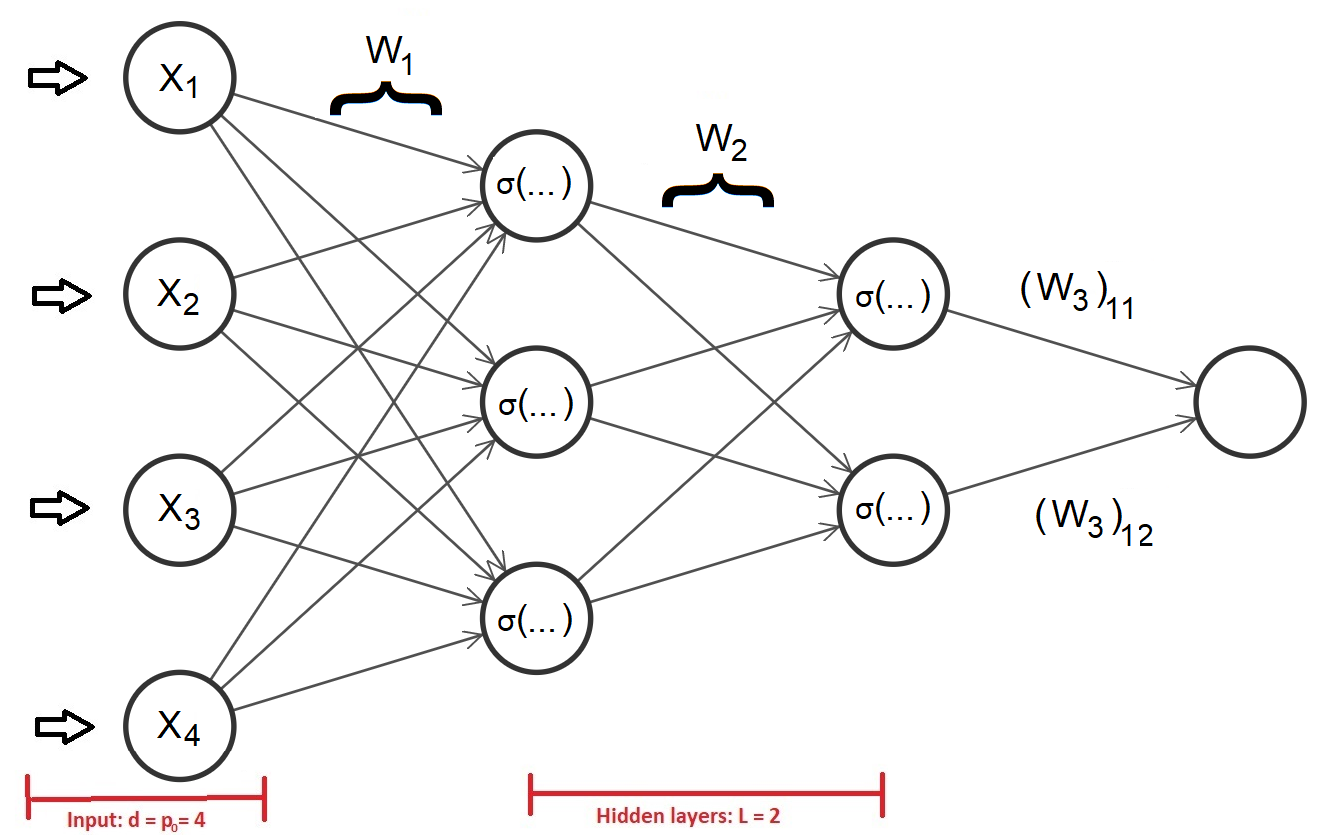
\includegraphics[width=8cm,height=8cm,keepaspectratio]{Bilder/NNGraphmitPfeilen1.png}
	\caption{Graphische Darstellung eines neuronalen Netzwerkes mit \textit{width vector} $\mathbf{p}=(4,3,2,1)$}
	\label{ungerichteterGraph}
\end{figure}
\end{frame}

\subsection{Rahmenbedingungen des Modells}
\begin{frame}
\begin{beamercolorbox}[sep=8pt,center,shadow=true,rounded=true]{title}
    \usebeamerfont{title}\insertsubsectionhead\par
\end{beamercolorbox}
\end{frame}

\subsubsection{Aktivierungsfunktion}
\begin{frame}
\frametitle{Aktivierungsfunktion}
\begin{figure}[h] % Do not use only [h] in real documents.
\begin{minipage}[t]{.45\linewidth}
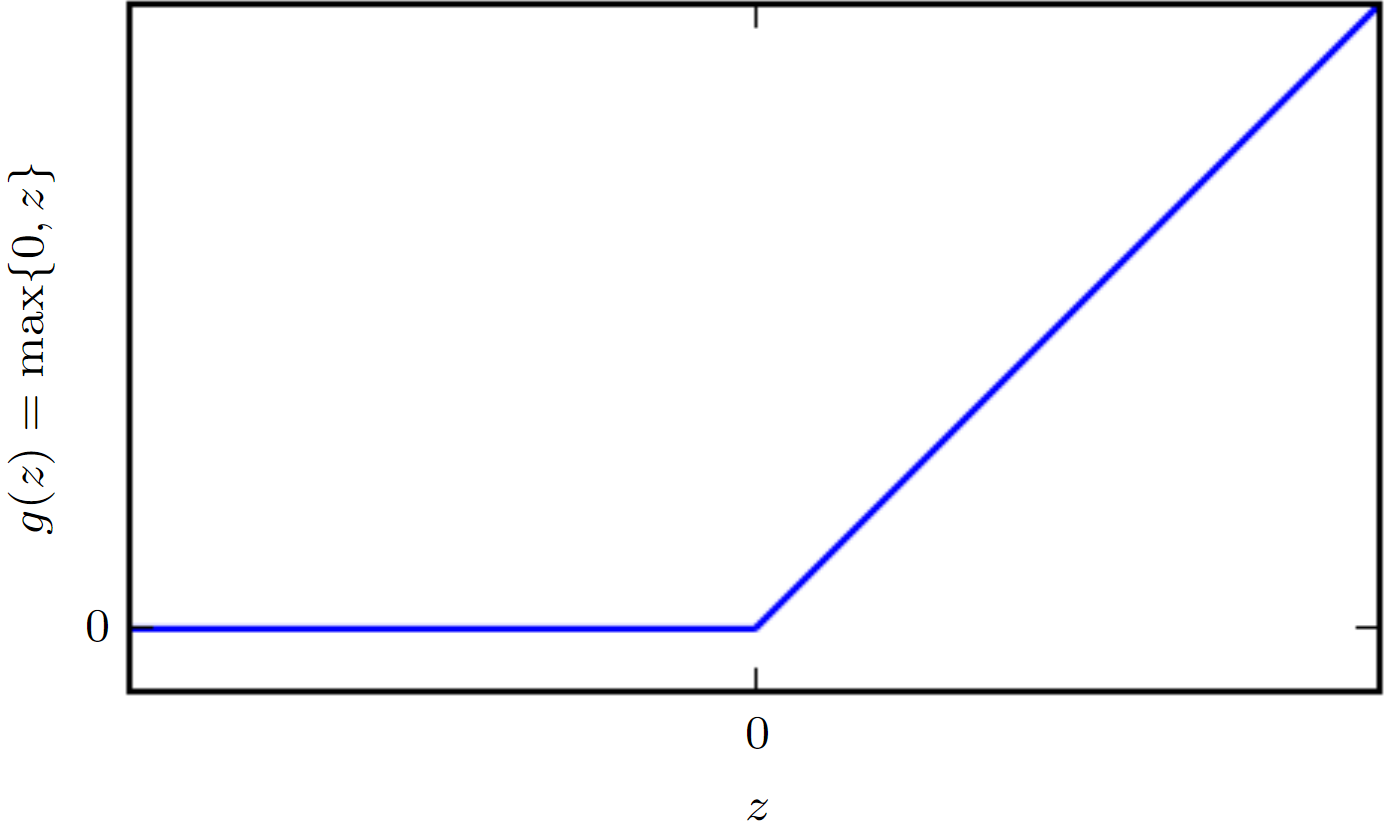
\includegraphics[width=0.8\textwidth]{Bilder/ReLU.png}
\caption[Caption for LOF]{Die ReLU Funktion}
\end{minipage}\hfill
\begin{minipage}[t]{.45\linewidth}
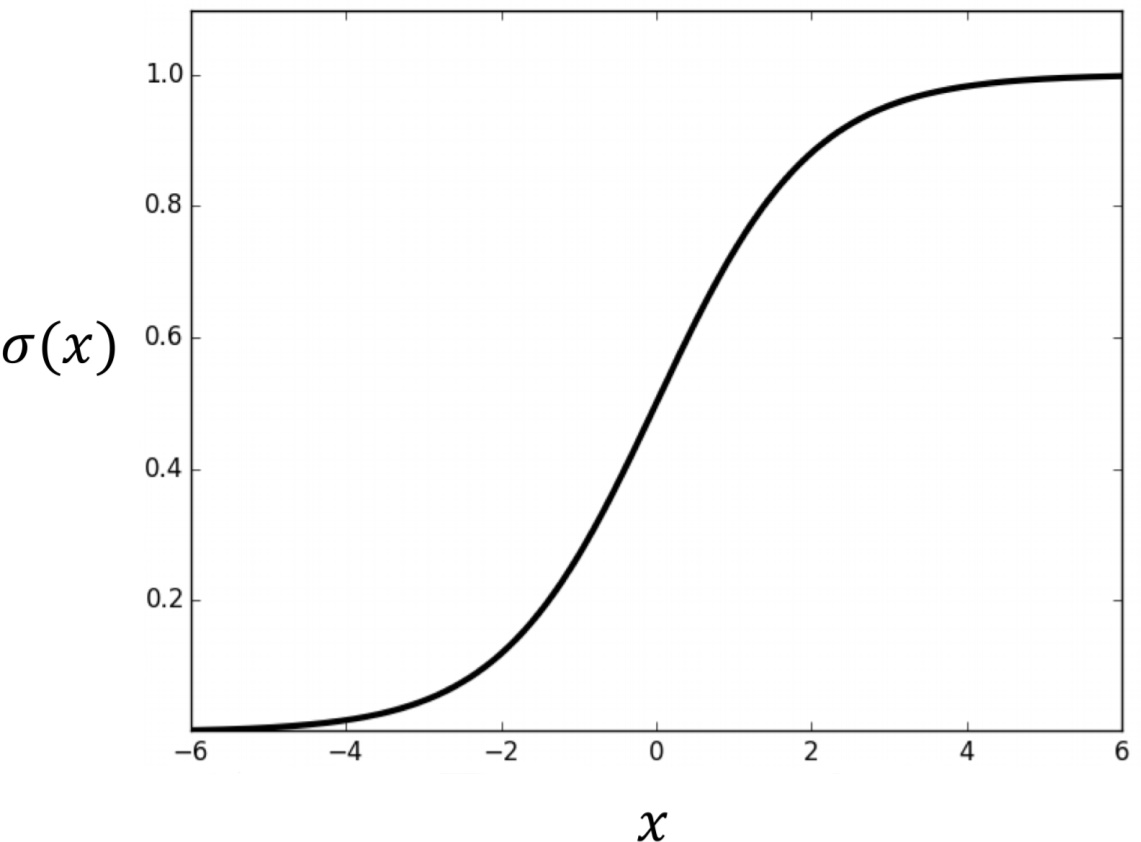
\includegraphics[width=0.8\textwidth]{Bilder/Sigmoid.jpg}
\caption[Caption for LOF]{Die Sigmoid Funktion}
\end{minipage}
\end{figure} 
\begin{itemize}
\item ReLU Aktivierungsfunktion: 
\begin{equation*}
\sigma: \mathbb{R} \to \mathbb{R};\quad  x \mapsto \sigma(x) = \max(0,x)  = (x)_+ 
\end{equation*}
\end{itemize}
\end{frame}


\begin{frame}
\frametitle{Aktivierungsfunktion: Vorteile ReLU \RN{1}}
\begin{itemize}
\item Produziert viele inaktive \textit{hidden units} \bigskip
\begin{figure}[h]
  \centering
  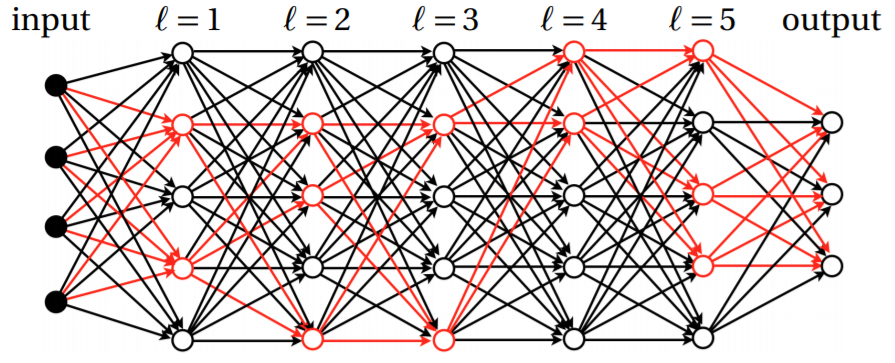
\includegraphics[width=0.7\textwidth]{Bilder/ReLUSparsity.png}
  \caption[Caption for LOF]{Ein \textit{sparse} Netzwerk mit ReLU Aktivierungsfunktion. Die roten Linien illustrieren die Verbindungen zu den aktiven Knoten.}
\end{figure}
\end{itemize}
\end{frame}

\begin{frame}
\frametitle{Aktivierungsfunktion: Vorteile ReLU \RN{2}}
\begin{itemize}
\item Häufiges Probleme bei anderen Aktivierungsfunktionen, ist das Problem des Verschwinden des Gradienten 
\begin{itemize}
\item[-] Stellt ein großes Hindernis im Lernalgorithmus dar und führt häufig zu Ungenauigkeiten des Modells
\end{itemize}
\item Nützliche Besonderheit der Funktion ist, dass sie eine Projektion ist
\begin{equation*} 
\sigma \circ \sigma = \sigma.
\end{equation*}
\end{itemize}
\end{frame}

\subsubsection{Netzwerkparameter}
\begin{frame}
\frametitle{Netzwerkparameter \RN{1}}
\begin{itemize}
\item Netzwerkparameter im Betrag kleiner $1$ halten, indem wir im Lernalgorithmus die Netzwerkparameter in jeder Iteration auf $[-1,1]$ projizieren: 
\begin{equation*}
F(L,\mathbf{p}) := \{f  \text{ in der Form \eqref{eq:1}}: \max\limits_{j = 0, ... ,L} \Vert W_j \Vert _{\infty}  \vee \vert \mathbf{v}_j \vert _{\infty} \leq 1 \}
\end{equation*}
\end{itemize}
\end{frame}

\subsubsection{Dünnbesetzte Parameter}
\begin{frame}
\frametitle{Dünnbesetzte Parameter \RN{1}}
\begin{itemize}
\item Größere Netzwerke können komplexere Aufgaben lösen, haben jedoch Neigung zum Overfitting \bigskip
\begin{figure}[h]
  \centering
  \includegraphics[width=0.5\textwidth]{Bilder/overfitting.pdf}
  \caption[Caption for LOF]{Problem des Overfittings durch tiefe neuronale Netzwerke ohne Regulierungen.}
\end{figure}
\end{itemize}

\end{frame}

\begin{frame}
\frametitle{Dünnbesetzte Parameter \RN{2}}
Lösungsansatz:
\begin{itemize}
\item Einführen von dünnbesetzten Netzwerkparameter
\item Falls $\Vert W_j \Vert _0$ die Anzahl der Nicht-Nullen Einträge von $W_j$ bezeichnet, dann definieren wir ein \textit{s-sparse} Netzwerk als 
\begin{equation*} 
\begin{split}
F(L,\textbf{p},s) &:= F(L,\textbf{p}, s, F) \\
                 &:= \{ f \in F(L,p): \sum_{j=0}^L \Vert W_j \Vert _0+ \vert \mathbf{v}_j \vert _0\leq s , \Vert \vert f \vert _\infty \Vert _\infty \leq F\}, 
\end{split}
\end{equation*}
\end{itemize}
\end{frame}

\subsubsection{Hierarchische Komposition der Regressionsfunktion}
\begin{frame}
\frametitle{Hierarchische Komposition der Regressionsfunktion \RN{1}}
\begin{itemize}
\item Für $\beta$-glatte Regressionsfunktion $f_0: [0,1]^d \rightarrow \mathbb{R}$ gilt eine Minimax-Konvergenzrate von $n^{-2 \beta /  2\beta + d}$
\item Müssen zusätzliche strukturelle Annahmen an die Regressionsfunktion treffen
\end{itemize}
\end{frame}

\begin{frame}
\frametitle{Hierarchische Komposition der Regressionsfunktion \RN{2}}
\begin{itemize}
\item Heuristische Idee: Performen gut bei komplexen Objekten, die durch einfache Objekte in einer iterativen Weise aufgebaut werden können \bigskip
\begin{figure}[h]
  \centering
  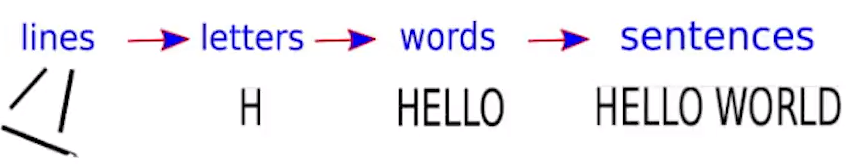
\includegraphics[width=0.5\textwidth]{Bilder/composition.png}
  \caption[Caption for LOF]{Beispiel einer hierarchischen Struktur: Aus Linien werden Buchstaben gebaut, aus Buchstaben werden Wörter geformt und zum Schluss werden die Wörter zu Sätzen zusammengesetzt.}
\end{figure}
\end{itemize}
\end{frame}

\begin{frame}
\frametitle{Hierarchische Komposition der Regressionsfunktion \RN{3}}
\begin{itemize}
\item Regressionsfunktion $f_0$, die aus einer Komposition von Funktionen besteht, das heißt 
\begin{equation*} 
f_0 = g_q \circ g_{q-1} \circ ... \circ g_1 \circ g_0
\end{equation*}
mit $g_i:[a_i, b_i]^{d_i} \rightarrow [a_{i+1}, b_{i+1}]^{d_{i+1}}$ 
\item Einzelnen Komponenten von $g_i$ bezeichnen wir mit $g_i = (g_{ij})_{j=1,...,d_{i+1}}^T$
\item $t_i \leq d_i$ als maximale Anzahl an Variablen, an denen die einzelnen $g_{ij}$ abhängen
\item Klassischer Ansatz: $g_{ij}$ in der Hölderklasse mit Glattheitsindex $\beta _i$
\end{itemize}
\end{frame}


\begin{frame}
\frametitle{Hierarchische Komposition der Regressionsfunktion \RN{4}}
Der Ball der $\beta$-Hölder Funktionen mit Radius $K$ ist definiert als 
\begin{align*}
C_r ^\beta (D,K) = \biggl\{ &f:  D \subset \mathbb{R}^r \rightarrow \mathbb{R} :  \\ 
&\sum _{\boldsymbol{\alpha}: \vert \boldsymbol{\alpha} \vert < \beta} \Vert \partial ^{\boldsymbol{\alpha}} f \Vert _\infty + \sum_{\boldsymbol{\alpha} : \vert \boldsymbol{\alpha} \vert = \lfloor \beta \rfloor} \sup_{\substack{\mathbf{x}, \mathbf{y} \in D \\ \mathbf{x}\neq \mathbf{y}}} \frac{\vert \partial ^{\boldsymbol{\alpha}} f(\mathbf{x}) - \partial ^{\boldsymbol{\alpha}} f(\mathbf{y}) \vert}{\vert \mathbf{x}-\mathbf{y} \vert _{\infty}^{\beta - \lfloor \beta \rfloor}} \leq K \biggr\},
\end{align*}
wobei $\partial ^{\boldsymbol{\alpha}} = \partial ^{\alpha _1}...\partial ^{\alpha _r}$ ein Multi-Index mit $\boldsymbol{\alpha} = ( \alpha _1, ..., \alpha _r) \in \mathbb{N}^r$  und $\vert \boldsymbol{\alpha} \vert := \vert \boldsymbol{\alpha} \vert _1$.
\end{frame}

\begin{frame}
\frametitle{Hierarchische Komposition der Regressionsfunktion \RN{5}}
Annahme: $f_0$ aus einer Komposition von Funktionen in der Klasse 
\begin{align*}
G (q,\mathbf{d}, \mathbf{t}, \boldsymbol{\beta}, K) := \{ & f_0 = g_q \circ ... \circ g_0: g_i = (g_{ij})_j: \\ & [a_i,b_i]^{d_i} \rightarrow [a_{i+1}, b_{i+1}]^{d_{i+1}}, \
g_{ij} \in C_{t_i} ^{\beta _i}([a_i,b_i]^{t_i},K), \\ &\text{für beliebige } \vert a_i \vert ,\vert b_i \vert \leq K \}
\end{align*}
mit $\mathbf{d} := (d_0, ..., d_{q+1}), \ \mathbf{t} := (t_0, ..., t_q), \ 	\boldsymbol{\beta} := (\beta _0,..., \beta _q)$ besteht.
\end{frame}

\subsection{Glattheit einer kompositionalen Funktion}
\begin{frame}
\frametitle{Glattheit einer kompositionalen Funktion}
\begin{itemize}
\item $f_0 = g_q \circ g_{q-1} \circ ... \circ g_1 \circ g_0$
\item Berechne Glattheit von $f_0$, die wiederum durch die Glattheit der Funktionen $g_i$ induziert wird
\item Sogenannte effektive Glattheitsindex 
\begin{equation*}
\beta _i ^* := \beta _i \prod \limits_{l= i+1}^{q}(\beta _l \wedge 1), \quad \quad \quad (\beta _l \wedge 1) := \min(\beta _l, 1)
\end{equation*}
\item 
$
\phi _n := \max \limits_{i=0,...q} n^{- \frac{2 \beta _i ^*}{2 \beta _i ^* + t_i}}.
$
\end{itemize}
\end{frame}

\subsection{Empirisches Risiko}
\begin{frame}
\frametitle{Empirisches Risiko}
\begin{itemize}
\item Gegeben $D_n = {(\mathbf{X}_1, Y_ 1, ..., \mathbf{X}_n,Y_n)}$, wobei $(\mathbf{X},Y), (\mathbf{X}_1, Y_ 1), ..., (\mathbf{X}_n,Y_n)$ u.i.v. Zufallsvariablen
\item Netzwerkfunktion $f$ konstruieren, sodass das empirische Risiko $ \frac{1}{n} \sum\nolimits_{i=1}^n (Y_i - f(\mathbf{X}_i))^2$ minimal ist
\item Für einen beliebigen Schätzer $\widehat{f}_n \in F(L,\mathbf{p},s,F)$ definieren wir 
\begin{align*}
\Delta _n (\widehat{f}_n, f_0) := \E _{f_0}\bigg[& \frac{1}{n} \sum_{i = 1}^n (Y_i - \widehat{f}_n(\mathbf{X}_i))^2 \\ &- \inf _{f \in F(L, \mathbf{p}, s,F)} \frac{1}{n}\sum_{i = 1}^n (Y_i - f(\mathbf{X}_i))^2 \bigg].
\end{align*}
\end{itemize}
\end{frame}

\section{Hauptresultat}

\theoremstyle{plain}
\newtheorem{thm}{Theorem}
\newcommand*{\theorembreak}{\usebeamertemplate{theorem end}\framebreak\usebeamertemplate{theorem begin}}
\subsection{Obere Schranke des L\textsubscript{2}-Fehler}
\begin{frame}[allowframebreaks]
\frametitle{Obere Schranke des $L_2$-Fehler}
\begin{thm} \label{thm:1}
Betrachte ein $d$-variates nichtparametrisches Regressionsmodell, wobei die Regressionsfunktion eine Komposition aus Funktionen besteht und dabei in der Klasse $G (q,\mathbf{d}, \mathbf{t}, \boldsymbol{\beta}, K)$ liegt. Sei nun $\widehat{f}_n$ ein Schätzer, der Funktionen in der Netzwerkklasse $F(L, (p_i)_{i = 0,..., L+1}, s, F)$ schätzt, wobei die Netzwerkklasse die folgenden Bedingungen erfüllt:
\theorembreak
\begin{itemize}
\item[(i)] Die zur Schätzung verwendeten neuronalen Netzwerke erlauben Funktionswerte, die mindestens so groß sind wie die maximalen Funktionswerte der Regressionsfunktion $f_0$: $F \geq \max(K,1)$ 
\item[(ii)] Für die Anzahl der Layer soll gelten: $\sum\nolimits_{i=0}^q \log _2(4t_i \vee 4 \beta _i) \log _2 n\leq L \lesssim n \phi _n$
\item[(iii)] Die Größe der Layer muss mindestens mit Rate $n\phi_n$ in $n$ gegen unendlich gehen: $n \phi _n \lesssim \min _{i = 1,...,L} p_i$
\item[(iv)] Anzahl der nicht verschwindende Einträge der Gewichtsmatrizen und Verschiebungsvektoren muss mit Rate $n \phi_n \log(n)$ in $n$ gegen unendlich gehen: $s \asymp n \phi _n \log n$
\end{itemize}
\theorembreak
Dann existieren Konstanten C und C', die nur abhängen von q, \textbf{d}, \textbf{t}, $\boldsymbol{\beta}, F$, sodass, wenn $\Delta _n(\widehat{f}_n, f_0) \leq C \phi _n L \log ^2(n)$ gilt, dann
\begin{equation} \label{eq:3}
R(\widehat{f}_n, f_0) \leq C' \phi _n L \log^2(n)
\end{equation}
und falls $\Delta _n (\widehat{f_n}, f_0) \geq C \phi _n L \log ^2 (n)$, dann 
\begin{equation} \label{eq:4}
\frac{1}{C'} \Delta _n(\widehat{f}_n, f_0) \leq R(\widehat{f}_n, f_0) \leq C' \Delta _n(\widehat{f}_n, f_0).
\end{equation}
\end{thm}
\end{frame}


\subsubsection{Folgerungen aus Theorem 1}
\begin{frame}
\frametitle{Folgerungen aus Theorem \RN{1}}
\begin{itemize}
\item Aus $\phi _n := \max \limits_{i=0,...q} n^{- \frac{2 \beta _i ^*}{2 \beta _i ^* + t_i}}$ können wir sehen, dass Rate nicht mehr von ursprünglichen Inputdimension $d$ abhängt, sondern von $t_i$
\item Aus der Bedingung \textit{(iv)} können wir folgern, dass wir ein \textit{sparse} Netzwerk vorliegen haben müssen
\item Flexible Möglichkeit eine gute Netzwerkarchitektur zu wählen, solange die Anzahl der aktiven Parameter $s$ die Bedingung $(iv)$ erfüllt
\end{itemize}
\end{frame}



\subsection{Untere Schranke des L\textsubscript{2}-Fehler}
\begin{frame}
\frametitle{Untere Schranke des $L_2$-Fehler}
\begin{thm} \label{thm zusatz}
Betrachte ein d-variates nichtparametrisches Regressionsmodell mit Beobachtungen $\mathbf{X}_i$ aus einer Wahrscheinlichkeitsverteilung mit einer Lebesque Dichte auf $[0,1]^d$, welche mit einer oberen und unteren positiven Konstante beschränkt ist. Für eine beliebige nicht-negative ganze Zahl q, beliebige Dimensionsvektoren \textbf{d} und \textbf{t}, die $t_i \leq \min (d_0,..., d_{i-1})$ für alle i erfüllen, ein beliebiger Glattheitsvektor $\boldsymbol{\beta}$ und alle hinreichend großen Konstanten $K > 0$, existiert eine positive Konstante c, sodass 
\begin{align*}
\inf_{\widehat{f}_n} \sup_{f_0 \in G(q,\mathbf{d},\mathbf{t}, \boldsymbol{\beta}, K)} R(\widehat{f}_n, f_0) \geq c \phi_n,
\end{align*}
wobei das $\inf$ über alle Schätzer $\widehat{f}_n$ genommen wird.
\end{thm}
\end{frame}

\begin{frame}
\frametitle{Untere Schranke des $L_2$-Fehler}
\begin{itemize}
\item Theorem \ref{thm:1} gibt uns obere Schranke für den $L_2$-Fehler für einen Schätzer aus der Netzwerkklasse $F(L,\mathbf{p},s, F)$ über der Klasse $G(q,\mathbf{d},\mathbf{t}, \boldsymbol{\beta}, K)$: 
\begin{equation*}
R(\widehat{f}_n, f_0) \leq C' \phi _n L \log^2(n)
\end{equation*}
\item Untere Schranke für $L_2$-Fehler über der Funktionsklasse $G(q,\mathbf{d},\mathbf{t}, \boldsymbol{\beta}, K)$:
\begin{equation*}
\inf_{\widehat{f}_n} \sup_{f_0 \in G(q,\mathbf{d},\mathbf{t}, \boldsymbol{\beta}, K)} R(\widehat{f}_n, f_0) \geq c \phi_n
\end{equation*}
\end{itemize}
\end{frame}


\subsection{Beweisidee zum Haupttheorem}
\begin{frame}
\frametitle{Einbettungseigenschaften einer Netzwerkfunktionsklasse}
\begin{itemize}
\item \textit{Größenvergleich} 
\item \textit{Komposition}
\item \textit{Layers hinzufügen/Netzwerktiefe angleichen} 
\item \textit{Parallelisierung}
\item \textit{Beseitigung der inaktiven Knoten}
\end{itemize}
\end{frame}


\begin{frame}
\frametitle{Approximationsqualität neuronaler Netzwerke \RN{1}}
\begin{small}
\begin{thm}
Für jede beliebige Funktion $h \in C_r^\beta ([0,1]^r, K)$ und jede beliebige ganze Zahl $m \geq 1$ und $N \geq (\beta + 1)^r \vee (K+1)e^r$, existiert ein Netzwerk 
\begin{equation*}
\widetilde{f} \in F (L, (r,6(r+\lceil\beta\rceil)N,..., 6(r+\lceil\beta\rceil)N, 1),s,\infty)
\end{equation*}
mit der Tiefe 
\begin{equation*}
L = 8 + (m + 5)(1+\lceil \log_2(r\vee \beta)\rceil)
\end{equation*}
und die Anzahl an Parameter 
\begin{equation*}
s \leq 141(r+\beta+1)^{3+r}N(m+6),
\end{equation*}
sodass 
\begin{equation*}
\Vert \widetilde{f} - h \Vert _{L^\infty([0,1]^r)} \leq (2K+1)(1+r^2+ \beta ^2)6^rN2^{-m}+K 3^\beta N^{- \frac{\beta}{r}}. 
\end{equation*}
\end{thm} 
\end{small}
\end{frame}


\begin{frame}
\frametitle{Approximationsqualität neuronaler Netzwerke \RN{2}}
\begin{itemize}
\item $f_0 = g_q \circ ... \circ g_0$ mit $g_{ij} \in C_{t_i}^{\beta_i} ([a_i,b_i]^{t_i}, K_i)$ und $K_i \geq 1$
\item $f_0 = g_q \circ ... \circ g_0 = h_q \circ ... \circ h_0$ mit \newline $h_{0j} \in C_{t_0} ^{\beta_0}([0,1]^{t_0},1)$ und \newline $ h_{ij} \in C_{t_i}^{\beta_i}([0,1]^{t_i},(2K_{i-1})^{\beta_i})$ für $ i = 1,..., q-1$ und $h_{qj} \in C_{t_	q} ^{\beta _q}([0,1]^{t_q}, K_q (2K_{q-1})^{\beta _q})$
\end{itemize}
\end{frame}

\begin{frame}
\begin{lemma}
Sei $h_{ij}$ wie oben definiert mit $K_i \geq 1$. Dann gilt für jede beliebige Funktion $\widetilde{h}_i = (\widetilde{h}_{ij})_j^\top$ mit $\widetilde{h}_{ij}:[0,1]^{t_i} \rightarrow [0,1],$
\begin{align*}
& \Vert h_q \circ ... \circ h_0 - \widetilde{h}_q \circ ... \circ \widetilde{h}_0 \Vert _{L^\infty [0,1]^d} \\
& \leq K_q  \prod\limits_{l=0}^{q-1} (2K_l)^{\beta _{l+1}} \sum\limits_{i=0}^{q} \Vert \vert h_i - \widetilde{h}_i \vert_\infty \Vert _{L^\infty[0,1]^{d_i}} ^{\prod_{l=i+1}^q \beta _l \wedge 1}. 
\end{align*}
\end{lemma} 
\end{frame}



\begin{frame}
\frametitle{Beweisidee zum Haupttheorem \ref{thm:1}}
\begin{itemize}
\item Für Stichprobenumfang $n \geq 3$ gilt:
\begin{align} \label{eq:5} 
\begin{split}
& \frac{1}{4} \Delta _n (\widehat{f}_n, f_0) - C' \phi_n L \log^2(n) \leq R(\widehat{f}_n , f_0) \\
& \leq 4 \inf\limits_{f^* \in F(L,\mathbf{p},s, F)} \left\Vert f^* - f_0 \right\Vert ^2 _\infty + 4\Delta_n(\widehat{f}_n , f_0) + C'\phi_n L \log^2(n).
\end{split} 
\end{align}
\end{itemize}
\end{frame}


\begin{frame}
\frametitle{Untere Grenze in \eqref{eq:4}}
\begin{itemize}
\item Falls $C \phi _n L \log^2(n) \leq \Delta _n (\widehat{f}_n,f_0)$ gilt und wir $ C= 8C'$ wählen, dann folgt für 
\begin{equation*}
C' \phi_n L \log^2(n) = \frac{1}{8} C \phi_n L \log^2(n) \leq \frac{1}{8}\Delta_n(\widehat{f}, f_0).
\end{equation*}
\item $R(\widehat{f}_n, f_0) \geq \frac{1}{8}\Delta_n(\widehat{f}_n, f_0)$
\end{itemize}
\end{frame}

\begin{frame}
\frametitle{Obere Grenze in \eqref{eq:3} und \eqref{eq:4}}
\begin{itemize}
\item Schranke für den Approximationsfehler $
\inf\limits_{f^* \in F(L,\mathbf{p},s, F)} \left\Vert f^* - f_0 \right\Vert_\infty$
\item Regressionsfunktion $f_0$ in der Form $f_0 = h_q \circ ... \circ h_0 $ mit $h_i =(h_{ij})_j ^\top, \ h_{ij}$ definiert auf $[0,1]^{t_i}$
\item Nach Theorem existiert Netzwerk $\widetilde{h}_{ij}$, sodass:\begin{equation} \label{eq:6}
\Vert \widetilde{h}_{ij} - h_{ij} \Vert _{L^\infty ([0,1]^{t_i} )} \leq (2Q_i +1 )(1+t_i^2+ \beta_i^2) 6^{t_i} N n^{-1} + Q_i 3^{\beta_i} N ^{- \frac{\beta_i}{t_i}}.
\end{equation}
\item Transformation des Output $x$ vom Netzwerk $\widetilde{h}_{ij}$ zu $(1-(1-x)_+)_+$ mit neuem Netzwerk $\sigma (h^*_{ij})$
\end{itemize}
\end{frame}

\begin{frame}
\frametitle{Obere Grenze in \eqref{eq:3} und \eqref{eq:4}}
\begin{itemize}
\item Es gilt $\sigma (h^*_{ij}) = (h^*_{ij} (\mathbf{x}) \vee 0 ) \wedge 1$ und 
\begin{equation*} 
\Vert \sigma (h^*_{ij}) - h_{ij} \Vert _{L^\infty ([0,1]^r)} \leq \Vert \widetilde{h}_{ij} - h_{ij} \Vert _{L^\infty([0,1]^r)}.
\end{equation*}
\item Durch Parallelisierung und Komposition erhält man $f^* = \widetilde{h}_{q1} \circ \sigma (h^*_{q-1} ) \circ ... \circ \sigma(h^*_0)$, wobei durch Hinzufügen von Layern, diese in Netzwerkklasse $F(L,\mathbf{p},s)$ liegt und die Bedingungen aus Theorem erfüllen
\end{itemize}
\end{frame}

\begin{frame}
\frametitle{Obere Grenze in \eqref{eq:3} und \eqref{eq:4}}
\begin{itemize}
\item $\inf\limits_{f^* \in F(L,\mathbf{p}, s)} \left\Vert f^* - f_0 \right\Vert_\infty^2 \leq C' \max\limits_{i=0,...,q} c^{- \frac{2\beta_i^*}{t_i}} n^{- \frac{2\beta^*_i}{2\beta^*_i + t_i}}$
\item Man kann zeigen, dass \begin{align*}
\inf\limits_{f^* \in F(L,\mathbf{p},s, F)} \left\Vert f^* - f_0 \right\Vert ^2 _\infty & \leq \inf\limits_{\widetilde{f} \in F(L,\mathbf{p},s)} 4 \Vert \widetilde{f} - f_0\Vert_\infty^2 \\
&\leq8 C \max_{i=0,...,q} c^{- \frac{2\beta^*_i}{t_i}} n ^{-\frac{2\beta_i^*}{2\beta_i^* + t_i}}.
\end{align*}
\end{itemize}
\end{frame}

\begin{frame}
\frametitle{Obere Grenze in \eqref{eq:3} und \eqref{eq:4}}
\begin{itemize}
\item Man kann folgern, dass
\begin{align*}
R(\widehat{f}_n , f_0) & \leq 4 \inf\limits_{f^* \in F(L,\mathbf{p},s, F)} \left\Vert f^* - f_0 \right\Vert ^2 _\infty + 4\Delta_n(\widehat{f}_n , f_0) + C'\phi_n L \log^2(n)\\
& \leq 32 C \max\limits_{i=0,...,q} c^{- \frac{2\beta_i^*}{t_i}} n^{- \frac{2\beta^*_i}{2\beta^*_i + t_i}} + 4 \Delta_n(\widehat{f}_n , f_0) + C' \phi_n L \log^2(n)
\end{align*}
\item Bedingung aus \eqref{eq:3}: $\Delta _n (\widehat{f}_n,f_0) \leq \widetilde{C} \phi _n L \log^2(n)$
\item Bedingung aus \eqref{eq:4}: $\Delta _n (\widehat{f}_n,f_0) \geq \widetilde{C} \phi _n L \log^2(n)$
\end{itemize}
\end{frame}




\end{document}
